\documentclass[portfolio.tex.tex]{subfiles}
\begin{document}

	\Chapter{Week 2}{Development Techniques}
		\section{Introduction}
			Last week we looked at web design using HTML, CSS and JavaScript. This week builds on this by introducing techniques for creating better webpages. These techniques include the best practice of \textbf{responsive design}, creating \textbf{user stories} in the design phase, and including \textbf{HTML Media tags} in the web page. \\

		\section{Weekly Content}
			\subsection{Responsive Design}
				Responsive design is all about modifying how your website looks based on the device. This is almost a mandatory practice now with the sheer number of users which primarily browse websites on their mobile device which come in all shapes and sizes. \\

				\subsubsection{Meta Viewport}
					The most important part of responsive design is also the easiest. Using the $<$meta name="viewport"$>$ tag in the head tag of the HTML file tells the browser to make the width of the page dependent on the width of the device, rather than the number of pixels on the screen. This is due to the high density of pixels on today's smartphones. \autocite{google-responsive}\\

					Adding the initial-scale=1 attribute to the meta tag will help with smartphones in landscape view.\autocite{google-responsive}\\

					Curious in the difference the meta viewport tag makes, I looked for examples of the difference. I found a side by side comparison on W3 Schools \autocite{viewport-example}:

					\fboxsep=1mm
					\fboxrule=5pt

					\hspace{-1cm}
					\splitpage{
						\centering
						\fcolorbox{black}{white}{					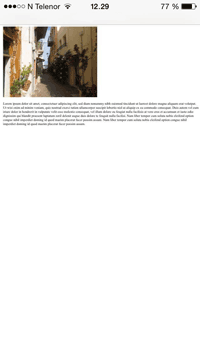
\includegraphics[width=0.6\textwidth]{img_viewport1.png}
						}
					\\
						\vspace{0.5cm}
							Without viewport.

					}{
						\centering
							\fcolorbox{black}{white}{					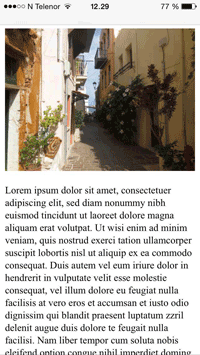
\includegraphics[width=0.6\textwidth]{img_viewport2.png}
							}
							\\
							\vspace{0.5cm}
							With viewport.
					}

				\subsubsection{Avoid Horizontal Scrolling}
					For a better user experience, only scroll vertically. This is what modern users are accustomed to, and scrolling horizontally or zooming to see a page properly will cause frustrations. \autocite{google-responsive}\\

				\subsubsection{Use Percentages for Size}
					For elements, it is preferred to assign size by percentage of parent element. This means that as the screen grows, so too does the element in proportion. Details such as margins, padding and font, should continue to use constant values.\\

				\subsubsection{Flexbox}
					Flexbox allows multiple elements within a row to be spread out various ways. Flexbox can evenly spread out these elements, or change the size of the elements proportionally to the row. When adding more elements, flexboxes will wrap around automatically. This creates a responsive design, while being very easy to develop by the developer. \\

				\subsubsection{Grid}
					CSS grid splits a container into grids. This allows for a container to be divided into the specified ratios. One part of this container is known as 1fr.  For example, if there was a container that had two children, one was 1fr, and the other was 3fr, the one child would take up 25\% of the space, and the other would take up 75\% of the space. See the example below:\\

					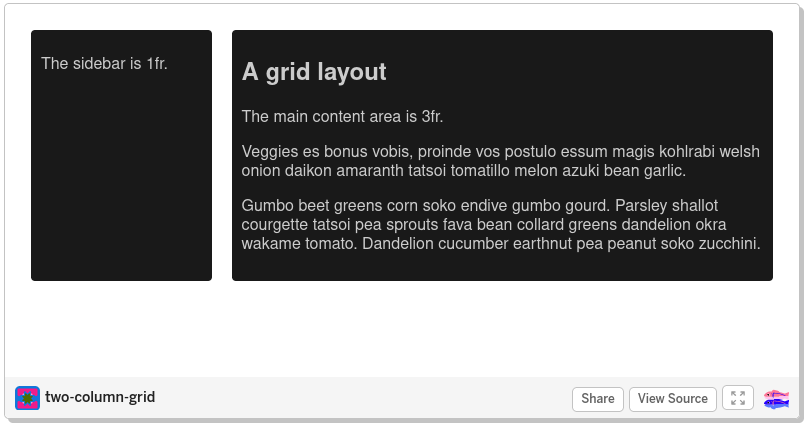
\includegraphics[width=10cm]{css-grid.png}

				\subsubsection{Media Queries}
					Media queries allow CSS to be specified depending on the screen size. This means that the same HTML and JavaScript can be used, while there are two completely different styles. Alternatively the two versions of the element could share many styles, and only differ with a few dimensions. Both scenarios are possible with media queries\\

					This allows the creation of "\textbf{breakpoints}" or points where the change in screen size, changes the layout of the page. Major breakpoints occur when there are significant layout changes, such as shifting from horizontal placement, to vertical. Minor breakpoints are where there is a shift in a smaller detail of the screen such as padding, or font-size. The syntax is as follows: \\

					\begin{lstlisting}
@media (max-width: 600px) {
	/* This CSS will be active for screens less than 600px wide*/
}

@media (min-width: 600px) {
	/* This CSS will be active for screens greater than 600px wide*/
}
					\end{lstlisting}
					\autocite{google-responsive}

			\subsection{User Stories}
				User Stories are a way of describing software requirements while skipping over the implementation details. It takes it a step further by placing the developer in the shoes of the user. This allows the developer to easily understand what is important to the user, how it will effect them and the urgency of the potential change. \\

				User stories can be written in the following formula:

				\begin{center}
					As a \underline{\textbf{user}}, I want \underline{\textbf{a feature}} so that I can \underline{\textbf{motivation}}
				\end{center}


				Different user personas can be specified so that distinct groups of users can be targeted (\textbf{who}), understanding \textbf{what} is important to them. These users will be connected to a specific feature, with a short explanation of \textbf{why} these features are important to these specific users.\\

				Although this formula shouldn't be a strict rule, and is more of a guideline for introducing the topic. The important part is that the sentence covers the \textit{who}, \textit{what}, and \textit{why}.\\

				User stories can also be broken up into three categories:

				\begin{enumerate}
					\item Epic Stories
						\subitem Large stories.
						\subitem General goals for the software.
						\subitem Usually the starting point for all user stories.
						\subitem Can be broken down into a few user stories.
					\item User Stories
					\item Sub Stories
						\subitem Small stories, usually smaller implementations that help with user stories.
				\end{enumerate}

			\vspace{0.5cm}
			\hspace{-0.5cm}
			\splitpage{
				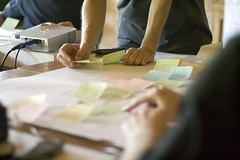
\includegraphics[width=0.8\textwidth]{posit-user-stories.jpg}
			}{
			These can be arranged in a table within a word document, but another, more interactive, method of writing out user stories within a physical location is Post-it notes. These can be colour coded based on size/priority. When a developer wants to implement a feature, they will grab a Post-it note and bring it to their desk, read and understand the requirements, and then write the implementation.

			}

			\subsection{HTML Media}
				Html Media tags are a way to add dynamic media into a website, instead of only static text and images. There are a few with varying uses:\\

				\hspace{-0.8cm}
				\begin{tabular}{|p{9cm}|p{6cm}|}
					\hline
					$<$video$>$ \newline
					$<$source src = "movie.mp4" type="video/mp4"$>$ \newline
					$<$/video$>$
					& Loads a local video, which can be either mp4 or ogg. Possible attributes on the video tag are controls, width, height, autoplay and muted, which are all fairly self-explanatory \autocite{w3-video}\\
					\hline
					$<$audio$>$ \newline
					$<$source src = "movie.mp3" type="video/mp3"$>$ \newline
					$<$/audio$>$&  Much the same as video, except the tag is audio instead of video. Uses mp3 instead of mp4, and does not have the height or width attributes. \autocite{w3-audio}\\
					\hline
					$<$canvas$>$& Creates a canvas on the screen which can then be drawn upon. This can be used to render graphics in real-time.  \\
					\hline
				\end{tabular}
			\subsection{HTML API}
				\subsubsection{Drag and Drop}
					An API that allows the developer to specify if an element is "draggable", and the actions that occur when that element is dropped. Most frequently the dropped element will be added as a child of the element it is dropped on. \autocite{w3-drag}\\

					A useful application of this feature might be for a ToDo list. Users will want to reorder the list so they can apply a manual priority for each task. Dragging and dropping is an intuitive way to do this.  \\

				\subsubsection{Geolocation}
					Accessible through JavaScript's navigator.geolocation which shares the users current location. Modern browsers will now ask the user if they would like to share their information, so this shouldn't be relied upon. \autocite{w3-geo}
		\section{Practical Tasks}
			\subsection{Task 1}
				\subsubsection{Reflection}
					Since I am just starting out in the web development, it is handy to investigate how other sites are built. I then can observe what works well from a user perspective, and what falls short. Taking this I am able to learn from it and adapt it into my own style for my own websites.

				\subsubsection{Introduction}
					Please see \ref{project-this-week} for further information about my proposal idea.

					Two websites I found to be similar were \textbf{Pinterest} and \textbf{garden.org}. Pinterest because they are an image driven, social website, and garden.org for the horticulture connection.

				\subsubsection{Pinterest}
					Pinterest as a large tech company and therefore has a good responsive design. \\

					\hspace{-0.8cm}
					\splitpage{
						Pinterest include the meta viewport tag in their header. \\

						They use a number of columns to display images. Wider the screen, the more columns there are on the screen. They keep these columns at a fixed width of 252 px, and change the margins of the page accordingly. The large container is styled using media tags, changing the width as necessary. Each element is loaded individually with JavaScript, and transformed/translated into place. The distances are calculated by knowing the previous images sizes as well as margins.
					}{
						\centering
						\vspace{0.3cm}
						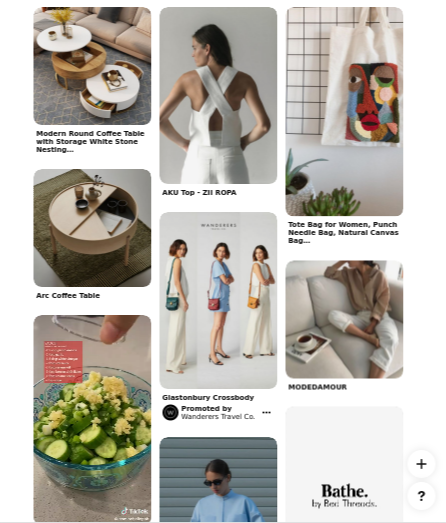
\includegraphics[width=0.8\textwidth]{pinterest-main-small}
					}

					\begin{center}
						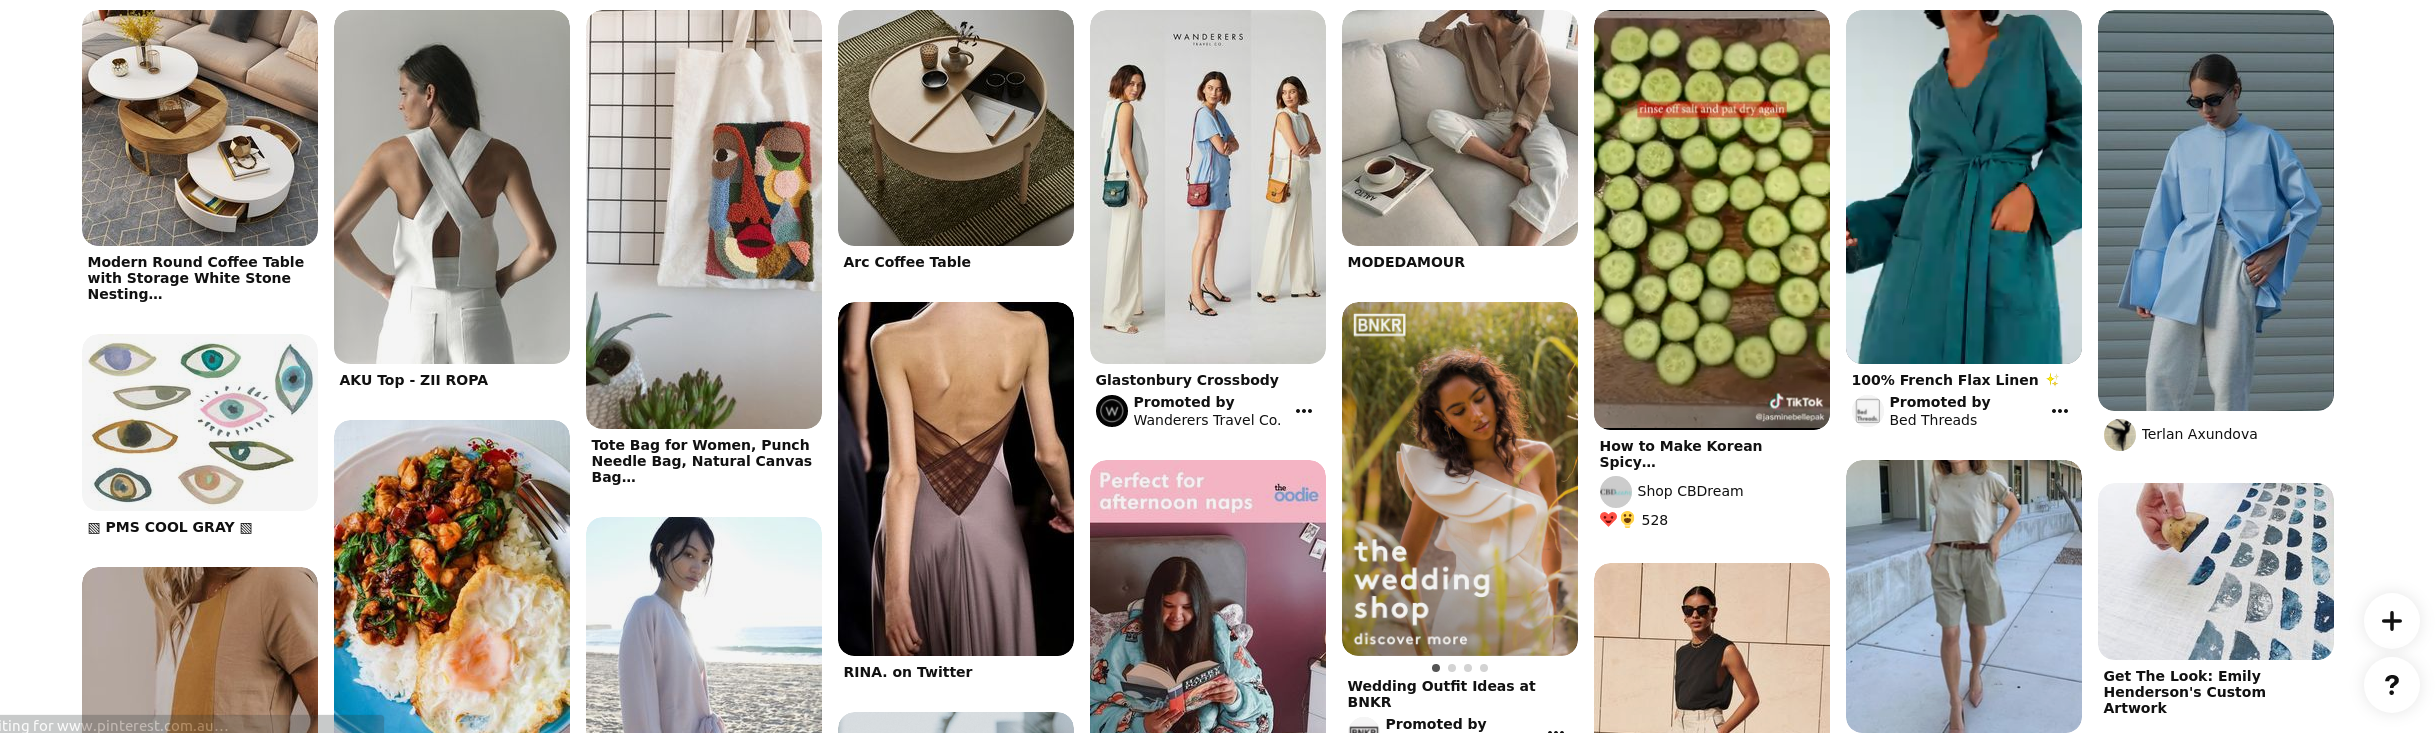
\includegraphics[width=15cm]{pinterest-main-large}\\

					\end{center}


					The navigation bar is also responsive. The main change is the search bar growing with the size of the screen to fill the navigation bar. Some features (such as advanced search) will disappear on lower widths when there isn't enough room. Finally on very small screens, the search bar becomes a button that users press to open up the search bar below.\\

					\begin{center}
						
\includegraphics[width=15cm]{pinterest-nav-large}\\
						
\includegraphics[width=8cm]{pinterest-nav-small}
					\end{center}

					On individual profile pages, the layout changes depending on the size of the screen. For smaller screens, the image/video is what you initially see, then scroll for the text/information. On larger screens, the image/video is on the left, while the information is on the right.

					\begin{center}
						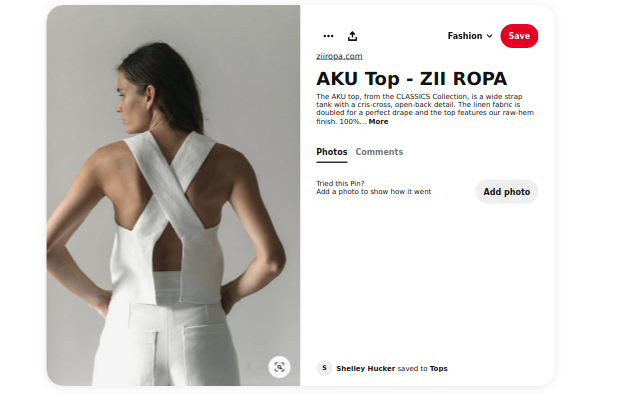
\includegraphics[width=10cm]{pinterest-item-large}\\
						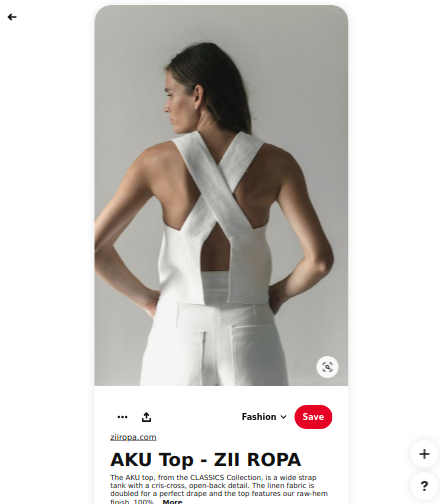
\includegraphics[width=6cm]{pinterest-item-small}
					\end{center}

				\subsubsection{garden.org}
					garden.org is also quite responsive. For larger screens ($>$ 1000px), there are two columns on the home screen, one for images  the other for comments. For smaller screens, there is only one column, with comments being below images. These two columns grow and shrink depending on the size of the screen. The images within these columns are in columns, and the number of columns changes based on the screen width.

					\begin{center}
						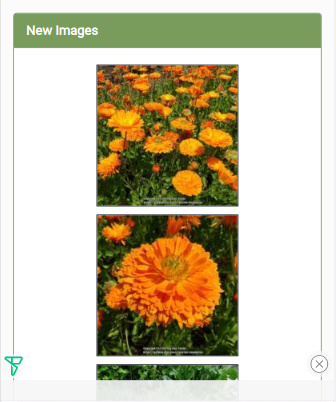
\includegraphics[width=7cm]{garden-one-small}
						\vspace{1cm}
						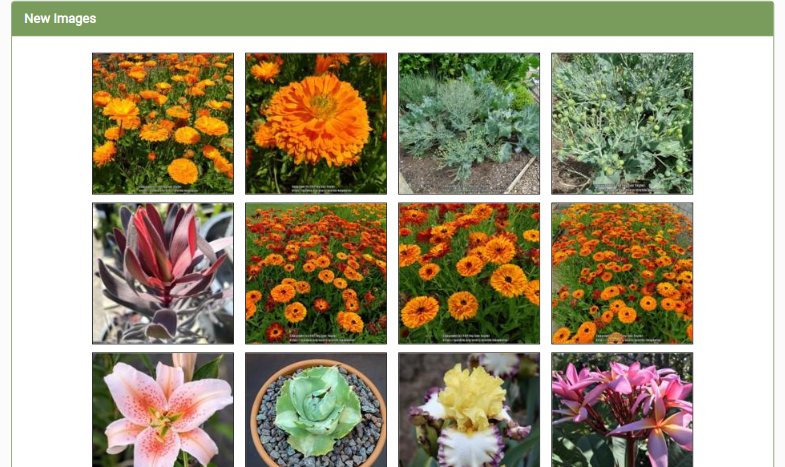
\includegraphics[width=7cm]{garden-one-large}\\
						\vspace{1cm}
						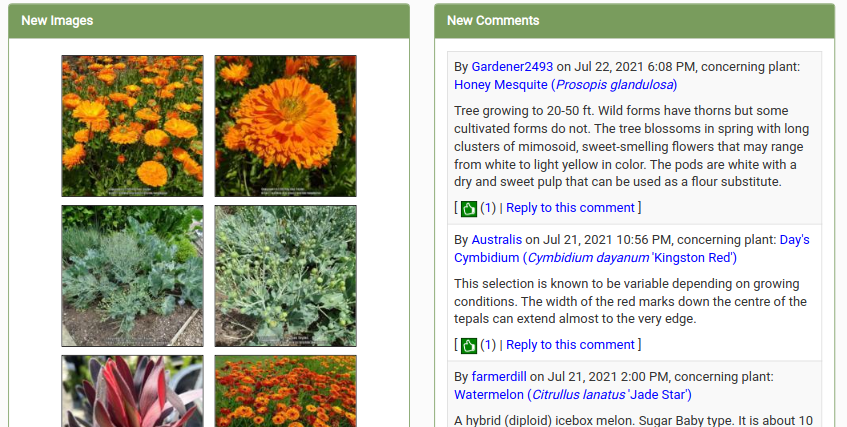
\includegraphics[width=10cm]{garden-two-small}\\
						\vspace{1cm}
						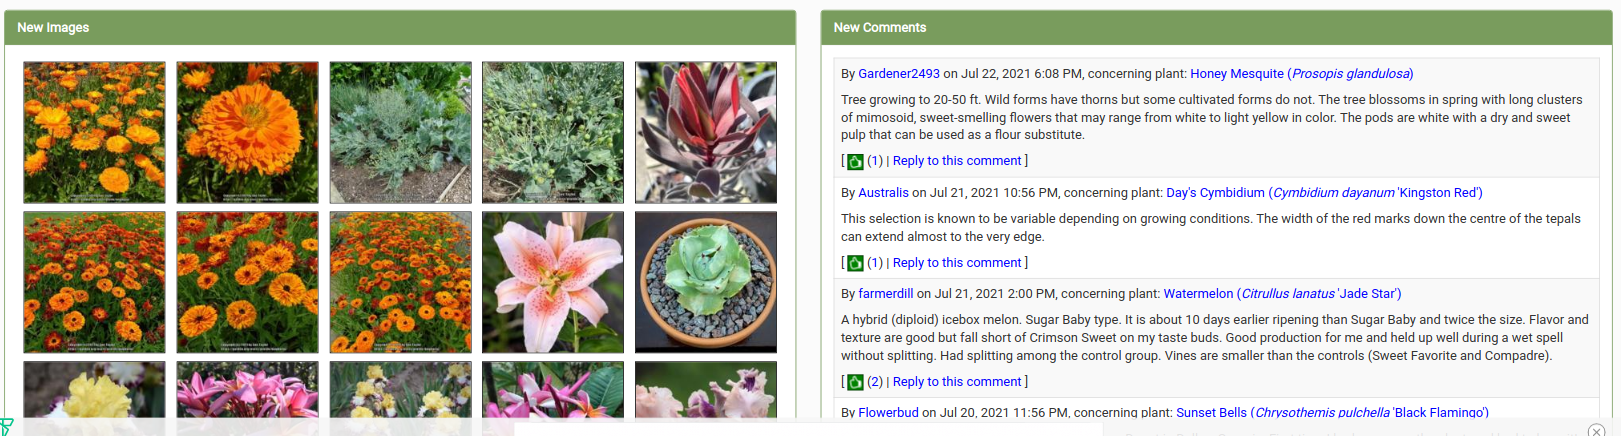
\includegraphics[width=14cm]{garden-two-large}\\
					\end{center}

					When clicking on an image, a pop up window appears containing a larger version of the image. This grows as the screen grows, when it reaches a certain point (~800px), it won't grow any more, but will stay centred in the screen.

					\begin{center}
						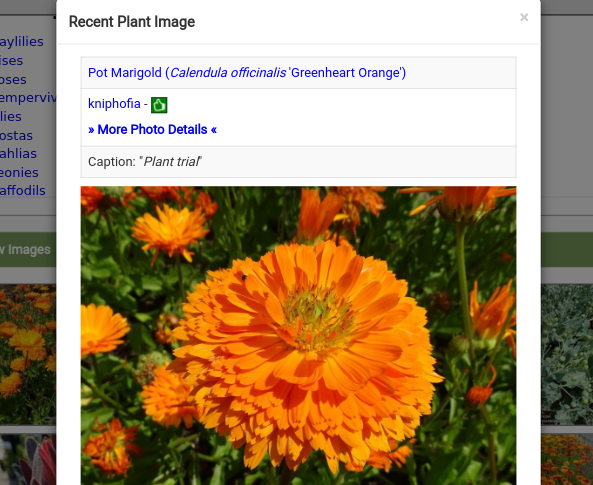
\includegraphics[width=7cm]{garden-pop-small}
						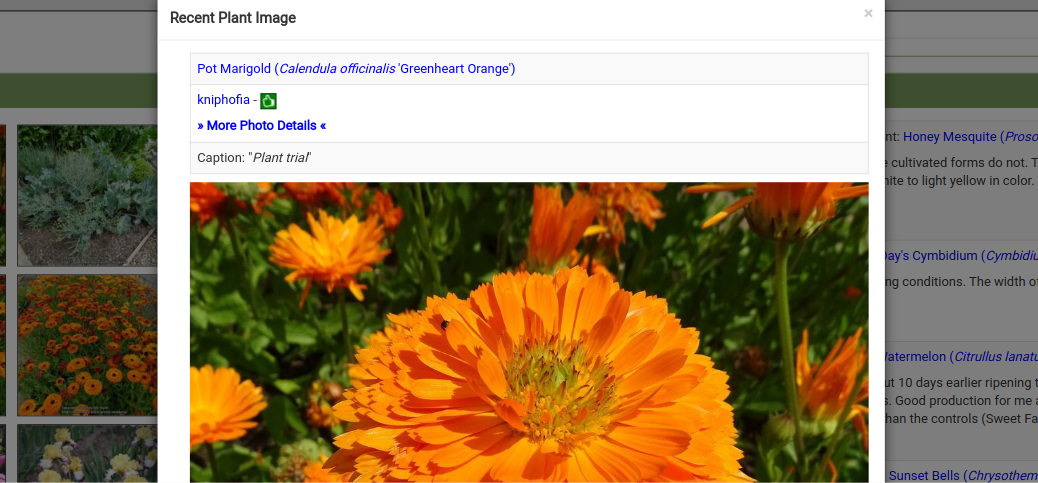
\includegraphics[width=7cm]{garden-pop-large}
					\end{center}

					garden.org has a much more of a grid-like feel compared to Pinterest since every image is the exact same size in the gallery. This leads to the website not feeling as fluid, even though it is still very responsive.

			\subsection{Task 2}
				\subsubsection{Reflection}
					Using CSS is the most efficient, and lightweight way to make a website responsive. Using the media tags, it is easy to create multiple versions of a design that adapts automatically. These also don't rely on the user having JavaScript enabled.

				\subsubsection{Screenshot}


					\splitpage{
						For Task 2, I decided to mock up the single plant page for my proposal. The information and photos just need to be added in later. I have created a simple layout of navigation bar at the top, as well as a main content pop-up in the middle of the screen. This will be overlayed on the screen as it's opened.  On a desktop ($>$1000px), the image will be on the left, and the text will be on the right. On a smaller device, the image will be prominent when the pop-up is opened, and the text will be below for the user to scroll through.\\

						There is another major breakpoint at 700px. Larger screens will have text in the navigation bar. Smaller screens will only have a search icon and a menu icon (which opens up a drop down menu with further options).
					}{
						\centering
						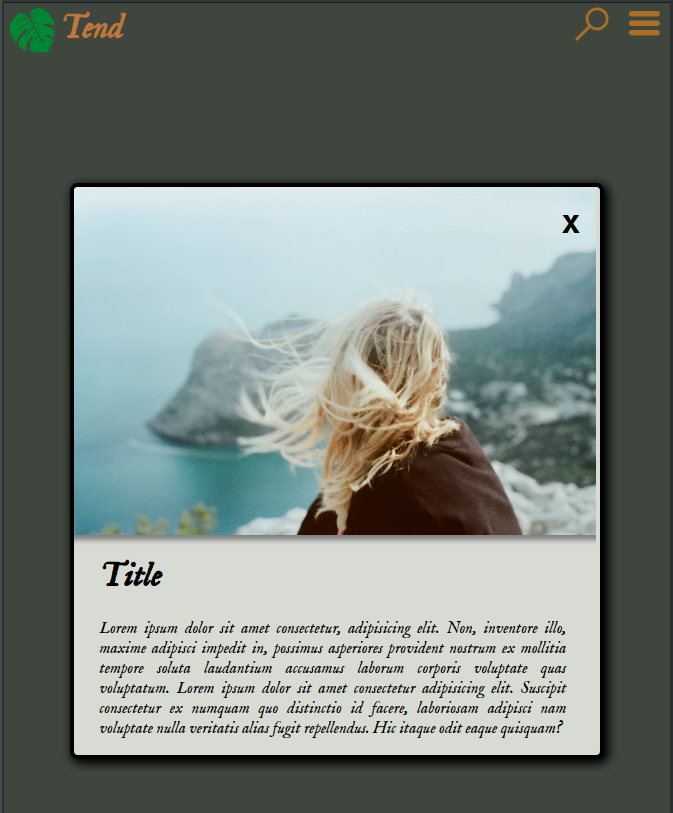
\includegraphics[width=0.9\textwidth]{tend-profile-small.png}\\
					}

					\begin{center}
						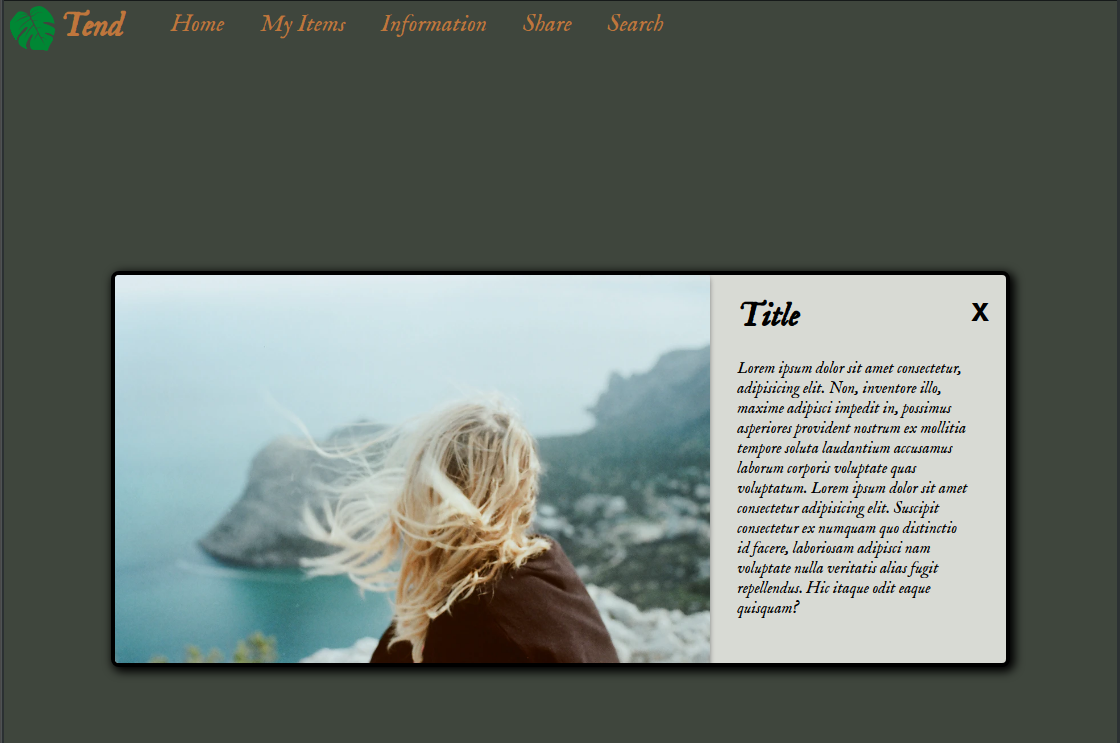
\includegraphics[width=12cm]{tend-profile-large.png}
					\end{center}


				\subsubsection{Source Code}
					For the source code go to \seqsplit{https://github.com/BrandonMurch/SIT120/tree/main/Practical\%20Tasks/Practical\%202/Task\%202}.

				\subsubsection{Useful Code}
					This task provided many useful bits of CSS codes to perform certain tasks. I would often find myself knowing what I wanted the website to look like, but not knowing how to do it. Some research led to the following code snippets.\\

					I wanted to create a more custom and identifiable appearance for my website., so I decided to use a custom font. I learned that the @font-face command needed to be used to incorporate a custom font. I downloaded my custom font locally, then used \ref{css-custom-font} to add it to the website.\\

					I also discovered another way to centre an element using flex-boxes.  \ref{css-center-element2}.\\

					Adding box shadows to my UI dramatically increased the visual appeal, creating a sense of depth for the user. \ref{box-shadow}.\\

					Since there were two edges of an image that touched the corners of a rounded container, I needed to individually round those two corners using \ref{specific-round-corners}.\\

					Since there was an inner element that needed to scroll, I wanted to modify the scrollbar. I used \ref{modify-scrollbar} to accomplish this.\\

			\subsection{Task 3}
				\subsubsection{Reflection}
					User stories are a very useful tool in the planning parts of software development. Putting yourself in the user's shoes to determine what is important to them, and what features need to be implemented help create understanding, as well as the ability to prioritise what is important for these users.\\

					Pre-designing UI within an application such as Figma saves a lot of time in the overall process. It is much easier to change a UI position, colour, etc.  in such a program, rather than rewrite the CSS in the actual web page each time. I found this out after spending a lot of time re-creating the first UI in Task 2, then noticing the difference using Figma in Task 3.\\

				\subsubsection{User Stories}
					\vspace{1cm}
					\begin{tabular}{p{6cm}|p{6cm}|p{4cm}}
						\large\textbf{Epic Stories} & \large \textbf{Acceptance Criteria \newline [Referenced User Story]} &\large \textbf{ Priority} \\
						\hline

						\textbf{Epic \#1:} As a person with many plants, I would like to be able to keep track of the schedules for these plants so they can be healthy.  &
						\vspace{-0.8cm}
						\begin{enumerate}
							\item  Create a plant profile. [1]
							\item 	Have the website generate a schedule based on the plant chosen, and be able to tweak that if necessary. [2]
							\item 	Notifications based on required scheduled events. [3]
						\end{enumerate}&

						\vspace{-1cm}\color{red}High\\

						\textbf{Epic \#2:} As a person who is new to horticulture, I would like to get new information about plants so that I am informed about how to care for them  &
						\vspace{-0.8cm}
						\begin{enumerate}
							\item   Search for information on specific plants. [4]
							\item 	Show new, useful tips. [5]
							\item 	Find general horticulture advice. [5]
						\end{enumerate}&

						\vspace{-1cm}\color{orange}Medium\\

						\textbf{Epic \#3:} As a social person, I would like to be able to share my plants, and interact with others, so that I am able to share experiences and ideas.  &
						\vspace{-0.8cm}
						\begin{enumerate}
							\item  	Discussion forum based on plant species. [6]
							\item 	Share photos of plants. [7,8]
							\item 	Interact with other users directly. [6]
						\end{enumerate}&

						\vspace{-1cm}\color{blue}Low\\

					\end{tabular}
					\vspace{2cm}
					\begin{tabular}{p{6cm}|p{6cm}|p{4cm}}
						\large\textbf{User Stories} & \large \textbf{Acceptance Criteria \newline [Reference Sub Story]} &\large \textbf{ Priority} \\
						\hline
%						\vspace{0.cm}
						\textbf{User Story \#1:} As a user, I would be able to create a plant profile so that I can store information about my plants.  &
						\vspace{-0.8cm}
						\begin{enumerate}
							\item  	Input information about plants. [1, 2]
							\item 	Upload image of plant. [1,2]
							\item 	Select species of plant. [1,2]
						\end{enumerate}&

						\vspace{-1cm}\color{red}High\\

%						\vspace{0.3cm}
						\textbf{User Story \#2:} As a user, I would like auto-generation of a schedule for my plants that I can adjust, so that I am able to see when I need to water/fertilize/re-pot my plants.  &

						\vspace{-0.8cm}
						\begin{enumerate}
							\item  	Auto-generate schedule based on species and climate. [2]
							\item 	Modify frequency of actions manually. [2]
							\item 	Regeneration of schedule if action occurs (Example: user waters plant). [3]
						\end{enumerate}&

						\vspace{-1cm}\color{red}High\\

						\textbf{User Story \#3:} As a user, I would like notifications about necessary actions so that I don't forget to water a specific plant.  &

						\vspace{-0.8cm}
						\begin{enumerate}
							\item  	Show notifications clearly.[3]
							\item 	Simple actions by clicking notifications. [3]
						\end{enumerate}&

						\vspace{-1cm}\color{red}High\\

						\textbf{User Story \#4:} As a user, I would like to be able to search for information on specific plants so that I am able to anticipate the level of care for a future plant, or properly care for a current plant.  &

						\vspace{-0.8cm}
						\begin{enumerate}
							\item  	Search For species of plant. [4]
							\item 	Get ideal schedule for specified plant. [5]
							\item 	Get trouble shooting guide for specific plant. [5]
						\end{enumerate}&

						\vspace{-1cm}\color{orange}Medium\\
					\end{tabular}
					\begin{tabular}{p{6cm}|p{6cm}|p{4cm}}
						\large\textbf{User Stories} & \large \textbf{Acceptance Criteria} &\large \textbf{ Priority} \\
						\hline

						\textbf{User Story \#5:} As a user, I would like to be shown new horticulture tips, so that I am able to learn about new topics and concepts.  &
						\vspace{-0.8cm}
						\begin{enumerate}
							\item  	Randomly display a tip of the day. [6]
							\item 	A "How-To" guide for basic horticulture principles and techniques. [7]
						\end{enumerate}&

						\vspace{-1cm}\color{orange}Medium\\

						\textbf{User Story \#6:} As a social user, I would like to discuss and exchange horticulture related ideas so I can expand my knowledge on more advanced topics, or ask more experience users for help.  &
						\vspace{-0.8cm}
						\begin{enumerate}
							\item  	Post to a discussion forum. [8]
							\item 	Message  users directly. [9]
						\end{enumerate}&

						\vspace{-1cm}\color{blue}Low\\
						\textbf{User Story \#7:} As a social user, I would like to share photos of plants I have grown so that I can proudly show off all my hard work  &

						\vspace{-0.8cm}
						\begin{enumerate}
							\item  	Add a photo to a plant profile. [2, 10]
						\end{enumerate}&

						\vspace{-1cm}\color{blue}Low\\

						\textbf{User Story \#8:} As a plant enthusiast, I would like to browse photos of other plants so that I can gain inspiration and enjoyment.  &
						\vspace{-0.8cm}
						\begin{enumerate}
							\item  	Browse other plant profiles. [11]
						\end{enumerate}&

						\vspace{-1cm}\color{blue}Low\\

					\end{tabular}

					\vspace{1cm}
					\hspace{-0.5cm}
					\begin{tabular}{p{6cm}|p{6cm}|p{4cm}}
						\large\textbf{Sub Stories} & \large \textbf{Acceptance Criteria} &\large \textbf{ Priority} \\
						\hline


						\textbf{Sub Story \#1:} As a user I would like to login or create an account so that I can store information for later.  &
						\vspace{-0.8cm}
						\begin{enumerate}
							\item  	Text input for username, password and a box to remember me.
							\item 	Button to register a new user.
								\subitem Able to input username, email, password
								\subitem After registration, user is asked to login with new credentials
							\item 	Successful login returns user to a personal home screen
						\end{enumerate}&

						\vspace{-1cm}\color{red}High\\

						\textbf{Sub Story \#2:} As a user I would like to  input information about my plants so that I can reference it later.  &
						\vspace{-0.8cm}
						\begin{enumerate}
							\item  	Text input for title, notes.
							\item 	Select species of plants using an autocomplete box.
							\item 	Upload image.
							\item 	Suggested water timings, fertilization and re-potting values which can be modified.
						\end{enumerate}&

						\vspace{-1cm}\color{red}High\\

						\textbf{Sub Story \#3:} As a user I would like to interact with my plants so I can record times I have watered, fertilized, etc..  &
						\vspace{-0.8cm}
						\begin{enumerate}
							\item  	Quick buttons for watering, fertilizing, re-potting.
							\item 	Generic action button for recording notes.
							\item 	Confirmation window to confirm actions in case of mistaken click.
						\end{enumerate}&

						\vspace{-1cm}\color{red}High\\
					\end{tabular}

					\begin{tabular}{p{6cm}|p{6cm}|p{4cm}}
						\large\textbf{Sub Stories} & \large \textbf{Acceptance Criteria} &\large \textbf{ Priority} \\
						\hline


						\textbf{Sub Story \#4:} As a user I would like to search for species of plants, so I can easily find what I am looking for.  &
						\vspace{-0.8cm}
						\begin{enumerate}
							\item  	Text input with autocomplete for searching.
							\item 	List relevant search results based on selected filters.
						\end{enumerate}&

						\vspace{-1cm}\color{orange}Medium\\

						\textbf{Sub Story \#5:} As a user I would like to get information for specific species. &
						\vspace{-0.8cm}
						\begin{enumerate}
							\item  	Display generic information
							\item 	Display usual watering schedule, humidity, and other care tips
							\item 	Display troubleshooting guide for an unhealthy plant
						\end{enumerate}&

						\vspace{-1cm}\color{orange}Medium\\

						\textbf{Sub Story \#6:} As a user I would like to get random tips of the day for plants that I am interested in.  &
						\vspace{-0.8cm}
						\begin{enumerate}
							\item 	Tip is based on a list of plants/topics which interest the user.
							\item 	Tip is displayed on the personal home screen.
						\end{enumerate}&

						\vspace{-1cm}\color{orange}Medium\\

						\textbf{Sub Story \#7:} As a user I would like to learn the basics of horticulture to ensure I am doing things correctly.  &
						\vspace{-0.8cm}
						\begin{enumerate}
							\item 	Written articles explaining certain topics.
							\item 	Browse all articles or search for specific
						\end{enumerate}&

						\vspace{-1cm}\color{orange}Medium\\

						\textbf{Sub Story \#8:} As a user I would like to post to the discussion forum so I can discuss and share ideas with others.  &
						\vspace{-0.8cm}
						\begin{enumerate}
							\item 	Browse previous posts based on topic
							\item 	Text box for writing the post.
							\item 	Click a button to submit the post
						\end{enumerate}&

						\vspace{-1cm}\color{blue}Low\\

					\end{tabular}

					\begin{tabular}{p{6cm}|p{6cm}|p{4cm}}
						\large\textbf{Sub Stories} & \large \textbf{Acceptance Criteria} &\large \textbf{ Priority} \\
						\hline

							\textbf{Sub Story \#9:} As a user I would like to message other users directly.  &
						\vspace{-0.8cm}
						\begin{enumerate}
							\item 	Click on users profile to message.
							\item 	Text box for writing the message.
							\item 	Click a button to submit the message
						\end{enumerate}&

						\vspace{-1cm}\color{blue}Low\\

						\textbf{Sub Story \#10:} As a user I would like to create a public profile for my plant.  &
						\vspace{-0.8cm}
						\begin{enumerate}
							\item 	Add public profile message to plant.
						\end{enumerate}&

						\vspace{-1cm}\color{blue}Low\\

						\textbf{Sub Story \#11:} As a user I would like to browse other plant photos.  &
						\vspace{-0.8cm}
						\begin{enumerate}
							\item 	Look at many different plant photos in an efficient way.
							\item 	Be able to find out more about plants that are interesting.
						\end{enumerate}&

						\vspace{-1cm}\color{blue}Low\\
					\end{tabular}



				\subsubsection{UI}
					I used Figma to design one of the pages for my application. I designed the "Share Plants" page from my proposed web app. I decided on a fairly neutral, and natural colour scheme. This was a change from the originally dark colours I was going to use for the website.  Thanks to Figma, this was a painless change.
					I was able to reuse my custom font from the earlier task with my new colour palate. \\

					The end result was:\\


					\begin{center}
						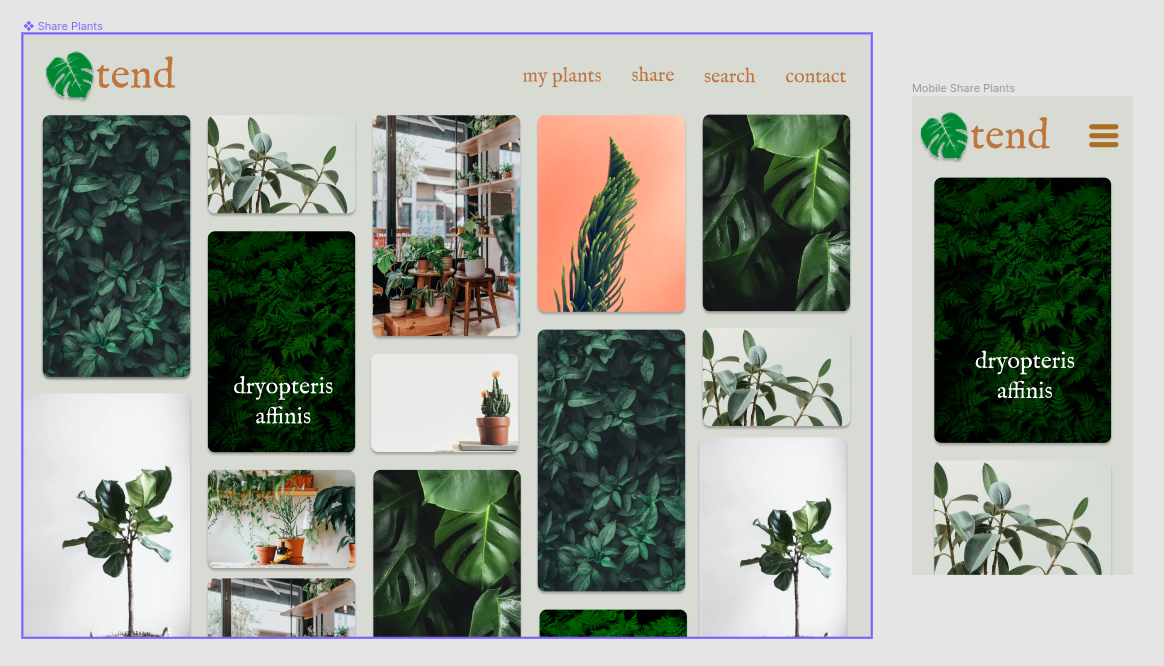
\includegraphics[width=0.8\linewidth]{share plants.png}
					\end{center}

					Much of this design can be reused throughout the web app, such as the navigation bar at the top, logo, etc. I will continue to use Figma to design the remaining pages of my web app before fully implementing them in Vue.\\

					I was able to get mock images from \link{https://www.unsplash.com}{unsplash.com}, which will be populated by real user images on the live version. The logo is a modified svg image from \link{https://www.pixabay.com}{pixabay.com}.

			\subsection{Task 4}
				\subsubsection{Reflection}
					This task was helpful to become familiar with some of the media tags. The canvas tag in particular, even though I have barely scratched the surface of what it can do. HTML has come such a long way from simply displaying text and is incredible what it can currently do just by itself.\\



					\splitpage{					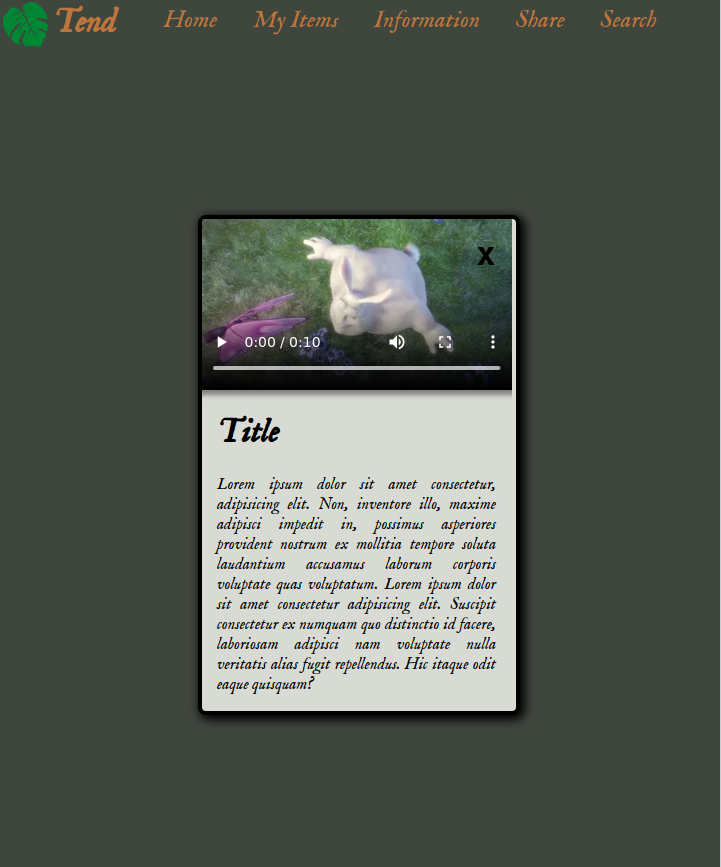
\includegraphics[width=0.9\textwidth]{task4-video.png}\\
					}{
					\subsubsection{Explanation of Task Work}

					For task 4, I decided to play around with the video and canvas tag. \\

					For the video tag, I used the previous template I was working on for my proposal site, but instead of an image, it had a video. This will allow users to be able to upload videos as well as pictures. Plant users love a good time lapse!\\
					}


					\vspace{0.5cm}

					\splitpage{
						I also used the canvas tool, as well as some JavaScript to animate a green wreath around an idle mouse. The design needs a little work aesthetically, but is a neat concept. This is achieved by finding the mouse with a "onmousemove" attribute on the canvas. This allows the position to be stored, and the countdown started. After an certain number of seconds the wreath begins forming. This makes use of the quadraticCurveTo, as well as some basic trigonometry/linear equations.\\
					}{
						\centering
						
\includegraphics[width=0.8\textwidth]{green-wreath.png}
					}

				\subsubsection{Source Code}
					For task 4 source code, see \seqsplit{https://github.com/BrandonMurch/SIT120/tree/main/Practical\%20Tasks/Practical\%202/Task4}.

				\subsubsection{Useful Code}
					Figuring out how to to draw a basic line on the canvas, I used \ref{js-canvas}.

					While playing around with the canvas, I tried to animate it by calling a function every x seconds to draw a new line. To accomplish this in JavaScript i used \ref{js-delay}.

		\section{Project}
			\subsection{This Week}
				\label{project-this-week}
				This week, I have come up with the basic idea for my web application. I will create an online website to store and share information about house plants. Part of the site will be a place to store information about current plants including water schedule, notes, etc. Another part will allow people to share experiences and photos of their plants. \\

				Also throughout this weeks tasks, I have created one of the pages necessary, as well as worked on the mock-ups and user stories.

			\subsection{Next Week}
				Next week I fill focus on finishing the proposal. This includes finishing the user stories, the proof of concept as well as the mock ups. I will then go over and review before submission. This should take approx. 8 hours.

\pagebreak

\end{document}